\documentclass[12pt]{article}

\usepackage[spanish]{babel}
\usepackage[utf8]{inputenc}
\usepackage{graphicx}
\usepackage{geometry}
\usepackage{xcolor}
\usepackage{fancyhdr}
\usepackage{lastpage}
\usepackage{pdfpages}
\usepackage{listings}

\geometry{top=25mm,left=15mm,right=15mm,a4paper}

\pagestyle{fancy}
\fancyhf{}
\lhead{Sistemas Operativos}
\cfoot{Página \thepage\ de \pageref{LastPage}}

\graphicspath{./}

\begin{document}
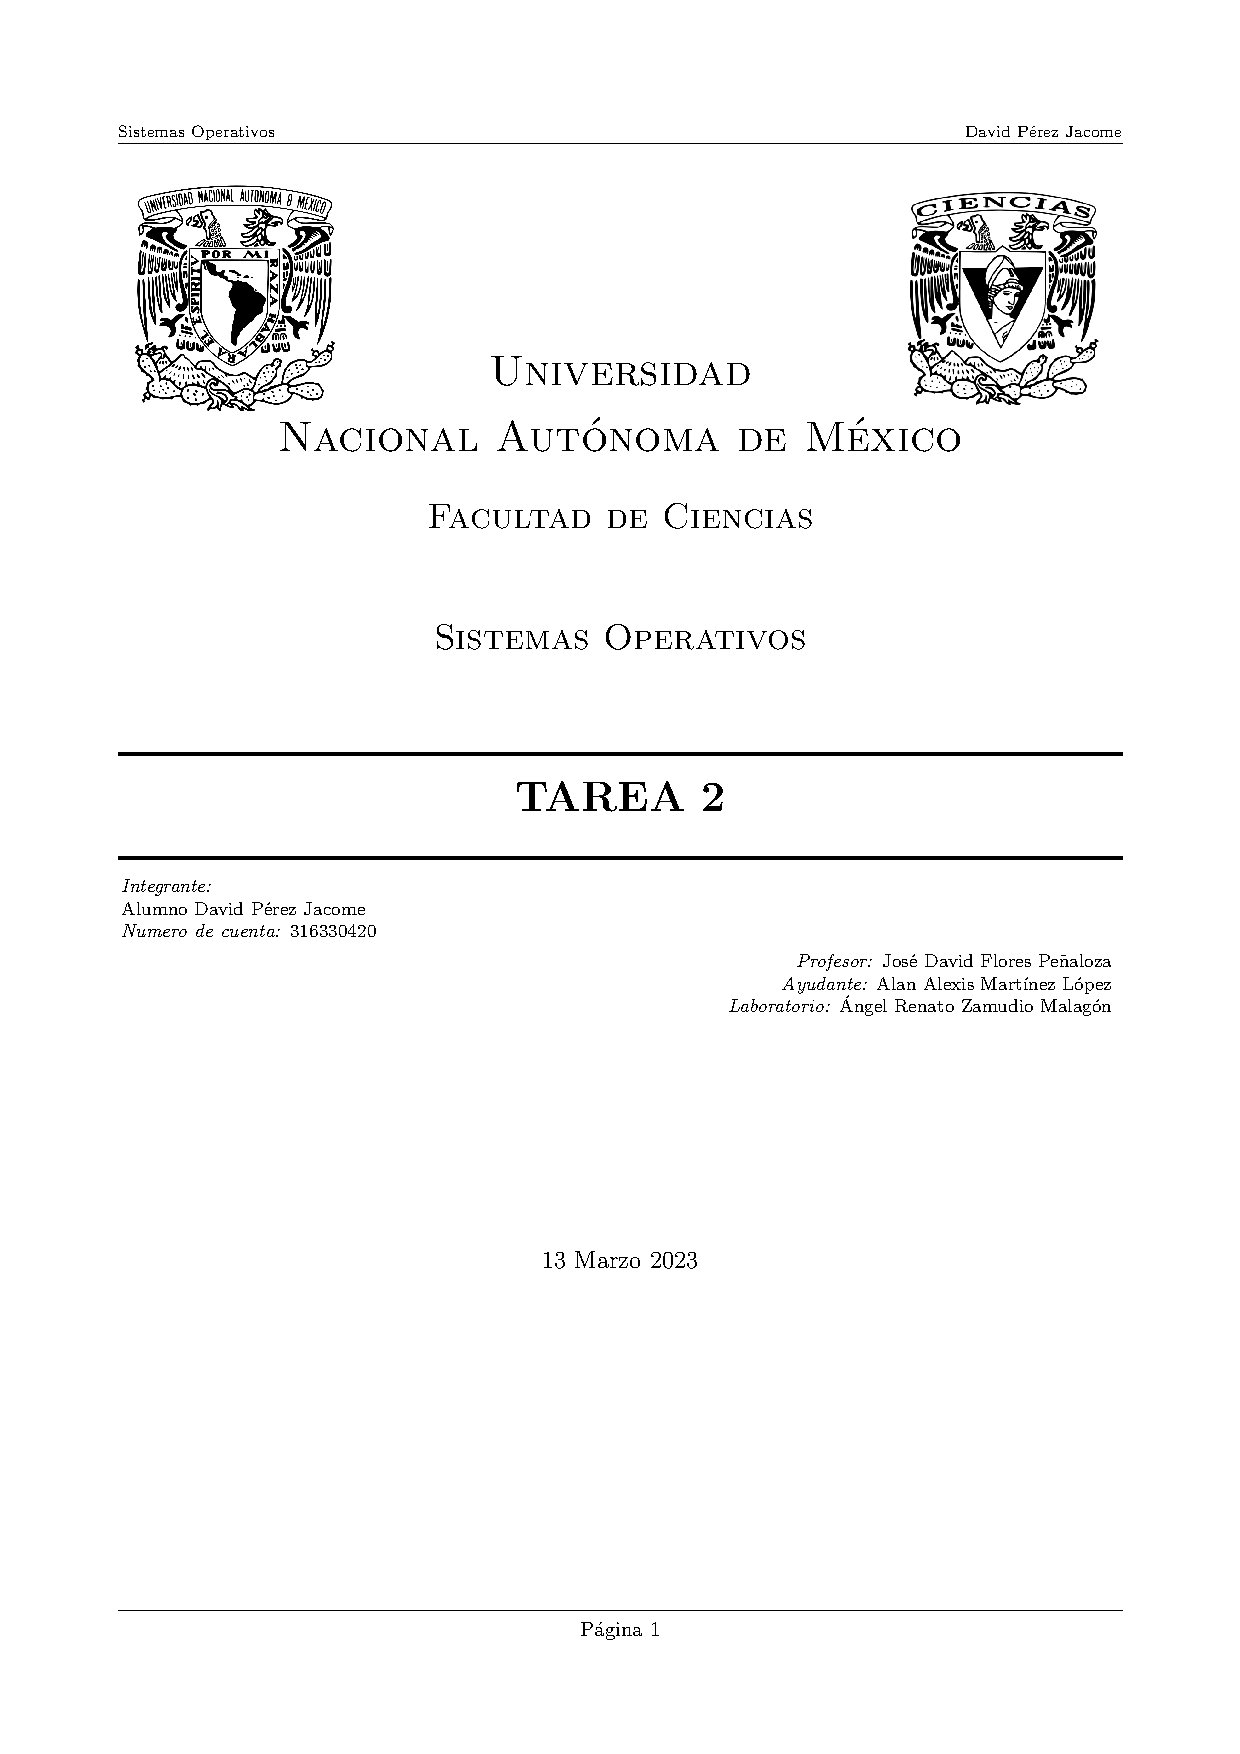
\includepdf{Portada.pdf}
{\color{blue} \section*{Tarea 2.}}

{\color{blue} \subsection*{Instrucciones.}}
\vspace{0.5em} 

Lee con atención las preguntas y contesta lo correspondiente. La tarea se entregará por vía classroom
en un archivo pdf que debe tener el nombre completo y número de tarea, ya sea en una portada o en el encabezado.
\textbf{La tarea se entregará de manera individual.}\\

{\color{blue} \subsection*{Ejercicios}}
\vspace{0.5em}

\begin{enumerate}
    \item ¿Qué es un proceso?
    \vspace{2mm}

    \textbf{resopuesta}

    \item ¿Cuál es la diferencia entre un programa y un proceso?
    \vspace{2mm}

    \textbf{respuesta}
    \item ¿Qué recuersos son necesarios para el correcto funcionamiento de un proceso?
    \vspace{2mm}

    \textbf{repuesta}
    \item ¿El procesador con que tipo de memoria puede trabajar exclusivamente?
    \vspace{2mm}

    \textbf{respuesta}

    \item Las llamadas a sistemas generalmente se hacen a través de una API ¿Por qué no hacemos llamadas al sistema invocándolas directamente?
    \vspace{2mm}

    \textbf{respuesta}

    \item ¿Qué es una maquina virtual?
    \vspace{2mm}

    \textbf{respuesta}
    \item Teniendo en cuenta que es una maquina virtual. ¿Qué es un sistema operativo anfitrión y qué es un sistema operativo húesped?  
    \vspace{2mm}

    \textbf{respuesta.}
    \item La maquina virtual de java ¿Es en realidad una maquina virtual? ¿De no ser así que es en realidad?
    \vspace{2mm}

    \textbf{respuesta}
    \item ¿Cuáles son los 3 estados que puede tener un proceso? Descríbelos
    \vspace{2mm}

    \textbf{respuesta} 
    \item ¿Qué es un proceso actual?
    \vspace{2mm}
    
    \textbf{respuesta}

\end{enumerate}

\end{document}